\chapter{何を解き、どこまで検証するのか}
\begin{chaptergoal}
\cgitem 分布関数と自己無撞着な電場の関係を理解する。\\
\cgitem 摂動の方程式に現れる二つの非線形項を導く。\\
\cgitem PDE（Partial Differential Equation：偏微分方程式）、有限次元ODE（Ordinary Differential Equation：常微分方程式）、量子アルゴリズムの検証範囲を区別する。
\end{chaptergoal}

\section{研究の全体像}
プラズマの運動論では、粒子の位置だけでなく速度の分布も追跡する。
分布関数 $f(\bm x,\bm v,t)$ は3次元位置・3次元速度の計6次元の変数を持つため、格子や基底を細かくすると自由度が急増する。
さらに、分布から電場を計算し、その電場が再び分布を変えるため、時間発展は非線形である。

対象研究の流れは、まずPDEをFourier--Hermite展開で二次ODEに変え、自由エネルギーに適合した座標を選び、Carleman階層に埋め込むというものである。
量子計算ではその線形系を扱い、最後に指定された物理的観測量を推定する。
図\ref{fig:workflow}は、現在のコードが担当する範囲も示している。
\begin{figure}[htbp]
\centering
\begin{tikzpicture}[node distance=7mm, every node/.style={font=\small},
 stage/.style={draw,rounded corners,align=center,text width=10.8cm,minimum height=9mm},
 >={Stealth}]
\node[stage] (pde) {非線形Vlasov--Poisson系（原論文：3D+3D）};
\node[stage,below=of pde] (ode) {Fourier--Hermite射影：$\dot\uu=F_1\uu+F_2(\uu\otimes\uu)$};
\node[stage,below=of ode] (lyap) {Lyapunov変換と振幅規格化：$\uu\mapsto\tu\mapsto\bu$};
\node[stage,below=of lyap] (car) {Carleman打ち切り：$\dot{\bm z}=A_C\bm z$};
\node[stage,below=of car,fill=blue!5] (quant) {量子演算子構成・量子ODEソルバ・観測量推定};
\draw[->] (pde)--(ode); \draw[->] (ode)--(lyap);
\draw[->] (lyap)--(car); \draw[->] (car)--(quant);
\end{tikzpicture}
\caption{理論から計算への流れ。現行コードは中間のODE・変換・Carlemanを1D1Vで検証する。}
\label{fig:workflow}
\end{figure}

\section{まず、何を計算する方程式なのか}
プラズマは、自由電子とイオンから構成される電離気体である。
通常の流体力学では密度、流速、温度などを計算するが、Vlasov方程式では、より詳細な粒子の位置と速度の分布を計算する。
例えば位置1次元・速度1次元なら、分布関数を $f(x,v,t)$ と書く。
これは時刻 $t$ に位置 $x$ 付近で速度 $v$ を持つ粒子がどのくらい存在するかを表し、微小領域の粒子数は $f(x,v,t)\,\dd x\,\dd v$ に対応する。
位置と速度を組み合わせた空間を\textbf{相空間}と呼ぶ。

\begin{figure}[htbp]
\centering
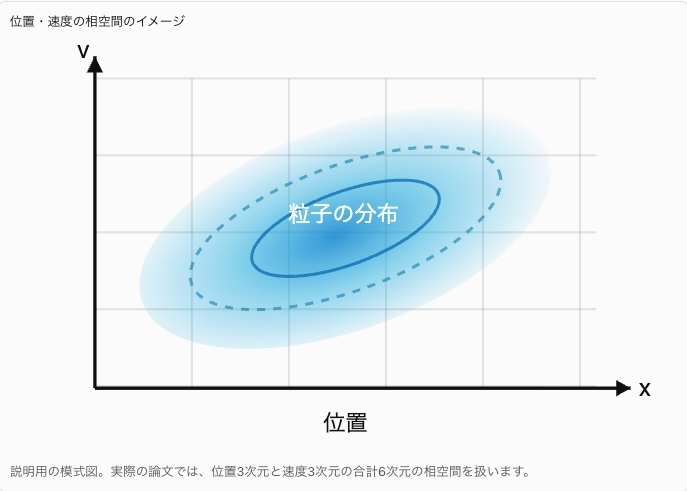
\includegraphics[width=.88\textwidth]{figures/phase_space.jpg}
\caption{位置・速度の相空間のイメージ。説明用の模式図であり、実際の論文では位置3次元と速度3次元の合計6次元の相空間を扱う。}
\label{fig:phase-space}
\end{figure}

分布関数を速度について積分すれば、密度や平均速度など、流体的な量を取り出せる。
1D1Vの場合、粒子密度 $n(x,t)$ と平均速度 $U(x,t)$ は
\[
n(x,t)=\int_{-\infty}^{\infty}f(x,v,t)\,\dd v,\qquad
U(x,t)=\frac{1}{n(x,t)}\int_{-\infty}^{\infty}v f(x,v,t)\,\dd v
\]
である（平均速度は $n>0$ の場所で定義する）。
3速度次元では積分を $\int_{\mathbb R^3}\dd^3v$ に置き換える。
Vlasov方程式を解くことで、密度だけでは区別できない速度分布の違いも追跡し、プラズマの波動、電場による加速、速度分布の変化などを調べられる。

\section{Maxwell分布と相対摂動 \texorpdfstring{$g$}{g}}
\subsection{平衡状態とは何か}
\textbf{平衡状態（equilibrium state）}とは、外部から新たな作用がなければ、時間が経過しても巨視的な状態が変化しない状態である。
本書で扱う論文では、特に空間的に一様で、平均流速がゼロのMaxwell速度分布を持つ状態を基準の平衡として採用する。

平衡状態でも、イオンは絶えずさまざまな方向へ運動し、その速度にはばらつきがある。
ある速度の粒子がある場所から出ていっても、周囲から同じ速度の粒子が入ってくれば、その場所の速度分布は変わらない。
個々の粒子は熱運動を続けていても、粒子全体の分布や密度・温度は時間的に変化しない。
したがって、平衡とは全ての粒子が静止することではない。

\subsection{平衡Maxwell分布とは何か}
Maxwell分布は、熱平衡にある粒子の速度分布を表す。
ここでは平均流速がゼロの平衡を考える。各速度成分はゼロを中心とするGaussian分布に従い、温度が高いほど分布の幅が広い。
これは速度ベクトルの分布であり、速さ $|\bm v|$ だけの分布とは区別する。
次元を持つ速度を $\bm V$ と書けば、イオンの平衡分布は
\[
f_0(\bm V)=n_0\left(\frac{m}{2\pi k_BT_i}\right)^{3/2}
\exp\left(-\frac{m|\bm V|^2}{2k_BT_i}\right)
\]
である。$n_0$ は平衡粒子密度、$m$ はイオン質量、$T_i$ はイオン温度、$k_B$ はBoltzmann定数で、$\int f_0\,\dd^3V=n_0$ を満たす。

熱速度 $v_{\mathrm{th}}=\sqrt{k_BT_i/m}$ を単位として $\bm v=\bm V/v_{\mathrm{th}}$ と置き、分布も $n_0/v_{\mathrm{th}}^3$ を単位として測る。
すると無次元の平衡Maxwell分布は
\begin{equation}
w(\bm v)=(2\pi)^{-3/2}\exp(-|\bm v|^2/2)
\label{eq:maxwell}
\end{equation}
となる。無次元とは、速度や分布を基準量との比で表すことで、物理単位を持たないという意味である。
この規約では $\int w\,\dd^3v=1$、各速度成分の分散は1であり、温度に由来する分布の幅は速度単位へ吸収されている。
温度の効果を取り除いたわけではなく、例えば後述する温度比 $\tau=T_i/T_e$ にも残る。

1速度次元への縮約では、対応する無次元平衡分布を
\[
\boxed{w_1(v)=\frac{1}{\sqrt{2\pi}}\ee^{-v^2/2}}
\]
と書く。図\ref{fig:maxwell-equilibrium}のように、速度0付近の粒子が多く、速度の絶対値が大きい粒子ほど少ない。
ただし、これは符号を持つ1成分の速度の分布であり、3次元の速さの分布を描いたものではない。
平衡状態ではこの分布の形が時間的に変化しない。

\begin{figure}[htbp]
\centering
% One-dimensional normalized Maxwell equilibrium (analytic curve).
\begin{tikzpicture}
\begin{axis}[
 width=.86\textwidth,height=5.8cm,
 xmin=-3,xmax=3,ymin=0,ymax=.45,
 xlabel={無次元速度 $v$},ylabel={平衡分布 $w_1(v)$},
 xtick={-3,-2,-1,0,1,2,3},ytick={0,.1,.2,.3,.4},
 grid=both,minor tick num=1,
 tick label style={font=\small},label style={font=\small}]
\addplot[blue!70!black,thick,domain=-3:3,samples=121]{exp(-x^2/2)/sqrt(2*pi)};
\end{axis}
\end{tikzpicture}

\caption{1速度次元の無次元Maxwell平衡分布。速度にはばらつきがあるが、平衡では曲線の形は時間に依存しない。表示範囲の外にも裾が続き、全速度での積分は1である。}
\label{fig:maxwell-equilibrium}
\end{figure}

\subsection{平衡からのずれを相対量で表す}
実際の分布を $f=f_0+\delta f$ と考え、平衡からの相対摂動を
\[
\boxed{g=\frac{f-f_0}{f_0}},\qquad \boxed{f=f_0(1+g)}
\]
と定義する。ここでは次元を持つ分布を使ったが、分子・分母を同じ単位で割れば比は変わらない。
以下では無次元化後の分布を改めて $f$ と書くので、同じ関係が $f=w(1+g)$ となる。

\begin{table}[htbp]
\centering
\caption{同じ位置・速度における $g$ の読み方。密度全体の増減率とは限らない。}
\begin{tabularx}{.92\textwidth}{lX}
\toprule $g$ の値 & 物理的な意味 \\\midrule
$0$ & 平衡分布と一致する。\\
$0.1$ & その位置・速度で平衡より10\%多い。\\
$-0.1$ & その位置・速度で平衡より10\%少ない。\\
$0.01$ & 平衡に対する1\%の小さな摂動である。\\
\bottomrule
\end{tabularx}
\end{table}

$g$ は無次元の相対的な分布の変化であり、密度そのものではない。
密度摂動は $g$ をMaxwell重み付きで速度積分した量である。
$g$ を用いると平衡は $g=0$ になり、平衡の周りの力学を一次項と二次項に整理し、Carleman線形化を適用しやすくなる。
ただし、点ごとの小さな $g$ と、後に用いるノルム条件 $R_P<1$ は同じ条件ではない。

\subsection{密度の揺らぎとKrook緩和}
1D1Vの場合は $f(x,v,t)=w_1(v)[1+g(x,v,t)]$ と書き、基準の平衡状態は
\[
\boxed{g(x,v,t)=0}
\]
である。一方、例えば周期領域で許される非ゼロ波数 $k$ に対して
\[
g(x,v,0)=0.1\cos(kx)
\]
とすると、$\int w_1\,\dd v=1$ より初期密度は
\[
n(x,0)=\int f(x,v,0)\,\dd v=1+0.1\cos(kx)
\]
となる。位置ごとに密度が平衡値より多かったり少なかったりするため、これは基準の一様平衡からずれた状態である。
この密度の揺らぎが電場を作り、その電場がさらに粒子の運動を変化させる。

後述するKrook緩和は、このような非平衡のずれを基準の平衡へ戻すモデルである。
輸送や電場など他の作用を無視すると、$\nuu>0$ の下で
\[
\partial_tg=-\nuu g,\qquad g(x,v,t)=g(x,v,0)\ee^{-\nuu t}
\]
なので、各位置・速度で
\[
\lim_{t\to\infty}g(x,v,t)=0,\qquad f(x,v,t)\longrightarrow w_1(v)
\]
となる。これは純粋な緩和だけを取り出した結論であり、一般の非線形発展には別途評価が必要である。

\subsection{平衡状態と定常状態の違い}
\textbf{定常状態（stationary state）}とは、時間が経過しても分布が変わらない状態である。
時間変化がないという性質だけでは、熱平衡にあるとは限らない。
例えば外部からエネルギーを供給し続けて一定の流れを維持する状態は、定常でも非平衡でありうる。

\begin{table}[htbp]
\centering\small
\caption{定常性、熱平衡、本書で採用する基準状態の区別。}
\begin{tabularx}{\textwidth}{lX}
\toprule 概念 & 意味 \\\midrule
定常状態 & 分布が時間に依存しない状態。外部駆動や流れがあっても定常になりうる。\\
熱平衡状態 & 熱力学的に平衡で、系と共に動く基準では持続的な熱流などがない状態。粒子の熱運動は続く。\\
本書の基準の平衡 & 平均流速ゼロの空間一様なMaxwell分布 $w(\bm v)$（1速度次元では $w_1(v)$）。\\
\bottomrule
\end{tabularx}
\end{table}

本書では、この特定の平衡を $g=0$ とすることがCarleman線形化への接続で重要になる。
平衡で時間微分がゼロになり、自己無撞着な電位もゼロになるため、Fourier--Hermite係数の方程式を
\[
\boxed{\dot\uu=F_1\uu+F_2(\uu\otimes\uu)}
\]
という定数項のない二次形式に整理できる。
Krook緩和によって平衡へ引き戻される効果と、非線形相互作用によって摂動が変わる効果を比較することで、後の章で収束の十分条件を導く。

\section{衝突付きVlasov方程式と自己無撞着な電位}
\sourcefile{HANDOVER.md} 第2節のモデルは、電子を断熱応答、イオンを運動論的に扱う、磁場なしの弱非線形プラズマである。
電子の密度応答は弱い電位について線形化し、イオン分布と電場の二次の相互作用を保持する。
空間は周期的で、衝突にはKrook型の緩和を用いる。
無次元方程式は
\begin{align}
\partial_t f&=-\bm v\cdot\nabla_x f
 +\nabla_x\phi\cdot\nabla_v f-\nuu(f-w),\label{eq:vlasov}\\
(\nabla_x^2-\tau)\phi&=-\int_{\mathbb R^3}g(\bm x,\bm v,t)w(\bm v)\,\dd^3v,
\qquad \tau=T_{\mathrm{ion}}/T_e>0.\label{eq:poisson}
\end{align}

式\eqref{eq:vlasov}は、分布 $f$ が空間輸送、電場加速、衝突緩和によってどう変わるかを表す。
符号を読みやすくするため、輸送と加速の項を左辺に移すと
\[
\partial_t f+\bm v\cdot\nabla_x f
+\bm a\cdot\nabla_v f=-\nuu(f-w),\qquad
\bm a=-\nabla_x\phi
\]
となる。衝突がなければ、粒子の軌道
\[
\frac{\dd\bm x}{\dd t}=\bm v,\qquad
\frac{\dd\bm v}{\dd t}=-\nabla_x\phi
\]
に沿って分布の値が運ばれる。
ここで $\phi$ は無次元静電ポテンシャルで、電場はこの規約で $\bm E=-\nabla_x\phi$ に対応する。
正のイオンに対する電荷・質量などの係数は無次元化に吸収されている。
右辺の $-\nuu(f-w)$ は、分布を基準のMaxwell分布へ戻す効果を表し、$\nuu>0$ は無次元緩和率である。

式\eqref{eq:poisson}は、分布から電位を決める遮蔽Poisson（Helmholtz）方程式である。
右辺の $\int gw\,\dd^3v$ は、平衡密度を1に規格化したときのイオン密度摂動である。
左辺の $-\tau\phi$ は電子の応答に由来する遮蔽を表す。
Fourier空間では、波数 $\bm k$ の密度摂動を $\rho_{\bm k}$ とすると
\[
\phi_{\bm k}=\frac{\rho_{\bm k}}{|\bm k|^2+\tau}
\]
となり、電位が密度摂動の線形汎関数であることがわかる。
分布から密度・電位を計算し、その電位を式\eqref{eq:vlasov}へ戻すため、この結合を\textbf{自己無撞着}と呼ぶ。
完全な平衡 $g=0$ なら、この周期系では $\phi=0$ である。
電位の符号や係数はこの無次元化に従い、別の規約を途中で混ぜると $F_1,F_2$ の符号も変わる。

\begin{notebox}
\textbf{「自己無撞着な電場」とは？}
粒子の分布が電場を決め、その電場が粒子の分布を変える関係を、矛盾なく同時に満たす電場のことである。
本モデルでは、各時刻の分布摂動 $g$ を速度について積分して密度摂動を求め、
式\eqref{eq:poisson}から電位 $\phi$、さらに電場 $\bm E=-\nabla_x\phi$ を計算する。
その電場による加速を式\eqref{eq:vlasov}へ入れて、分布を時間発展させる。
\[
\text{粒子分布}\ \longrightarrow\ \text{密度・電場}
\ \longrightarrow\ \text{粒子分布の変化}
\]
「自己」は粒子自身の分布が電場の源になること、
「無撞着」は分布から求めた電場と、分布の時間発展に使う電場が整合することを意味する。
ここでは電子の応答も遮蔽項を通じて含まれている。
このように、Vlasov方程式と遮蔽Poisson方程式を結合した問題として解く。
\end{notebox}

\subsection{相対摂動の方程式を導く}
式\eqref{eq:maxwell}より $\nabla_vw=-\bm v w$ なので、$f=w(1+g)$ の速度微分は
\[
\nabla_vf=(\nabla_vw)(1+g)+w\nabla_vg
=w\{-\bm v(1+g)+\nabla_vg\}
\]
である。$w$ は位置と時間に依存しないため、$\partial_tf=w\partial_tg$、$\nabla_xf=w\nabla_xg$ となる。
これらを式\eqref{eq:vlasov}へ代入し、$w$ で割ると
\begin{equation}
\boxed{\partial_tg=-\bm v\cdot\nabla_xg-\bm v\cdot\nabla_x\phi
 -(\bm v\cdot\nabla_x\phi)g+\nabla_x\phi\cdot\nabla_vg-\nuu g.}
\label{eq:g}
\end{equation}
五つの項は、空間輸送、平衡分布への電場作用、二つの非線形電場作用、衝突緩和に対応する。

\section{五つの項の物理的な意味}
\begin{table}[htbp]
\centering\small
\caption{式\eqref{eq:g}の各項。次数の分類は自己無撞着な電位 $\phi[g]$ を用いた場合である。}
\begin{tabularx}{\textwidth}{lXXc}
\toprule 項 & 名前 & 物理的な意味 & 次数 \\\midrule
$-\bm v\cdot\nabla_xg$ & 自由輸送 & 速度に従って粒子が移動する。 & 一次\\
$-\bm v\cdot\nabla_x\phi$ & 平衡分布への電場作用 & 電場が平衡速度分布を変形する。 & 一次\\
$-(\bm v\cdot\nabla_x\phi)g$ & 非線形電場作用① & 電場が既存の摂動分布にも作用する。 & 二次\\
$+\nabla_x\phi\cdot\nabla_vg$ & 非線形電場作用② & 加速が速度分布を移動・変形させる。 & 二次\\
$-\nuu g$ & 衝突緩和 & 摂動を平衡へ戻す。 & 一次\\
\bottomrule
\end{tabularx}
\end{table}

\subsection{第1項：自由輸送と位相混合}
電場と衝突がない1D1V系を考えると、
\[
\partial_tg=-v\partial_xg,\qquad
\partial_tg+v\partial_xg=0
\]
であり、解は
\[
\boxed{g(x,v,t)=g(x-vt,v,0)}
\]
である。速度 $v$ の分布は、その速度で空間を移動する。
例えば無次元速度 $v=2$ の成分は、無次元時間 $t=3$ で位置が6だけ進む（周期領域では位置を $L$ ごとに同一視する）。
異なる速度成分は異なる速さで進むため、相空間の分布はせん断され、位置を固定して見ると速度方向に細かな構造ができる。
これがphase mixing（位相混合）の基本である。
例えば初期状態が $g(x,v,0)=A\cos(kx)$ なら $g(x,v,t)=A\cos(kx-kvt)$ となり、速度に関する振動が時間とともに細かくなる。

\subsection{第2項：平衡分布への電場作用}
$-\bm v\cdot\nabla_x\phi$ は、電場が平衡Maxwell分布へ作用することから生じる。
実際、元の加速項の平衡部分は
\[
\frac{1}{w}\nabla_x\phi\cdot\nabla_vw=-\bm v\cdot\nabla_x\phi
\]
である。正のイオンが電場で加速されると、平衡速度分布からのずれが生まれる。
外から空間的に変化する電場を与える問題なら、初めに $g=0$ でもこの作用で摂動が生じる。
ただし本モデルの電位は外から任意に与えるものではなく、式\eqref{eq:poisson}で密度から決まる。
したがって全空間で $g=0$ の完全な平衡では $\phi=0$ となり、自発的に摂動が生まれるという意味ではない。
$\phi[g]$ が線形なので、この項も $g$ に関して一次である。

\subsection{第3項：電場と既存の摂動の相互作用}
$-(\bm v\cdot\nabla_x\phi)g$ は、第2項にさらに $g$ が掛かった項である。
$\nabla_v\{w(1+g)\}$ のうち $(\nabla_vw)g$ に由来し、電場が平衡から変形した分布へ作用する一部を表す。
電位は $g$ に対する線形な写像なので、電場と摂動の積は二次になる。
ここで「線形な写像」とは非局所的な速度積分・空間逆演算を含むことであり、各点で単純に $\phi=Cg$ とする意味ではない。

\subsection{第4項：加速による速度分布の移動・変形}
$+\nabla_x\phi\cdot\nabla_vg$ は、摂動自身の速度微分に由来する。
粒子の加速度 $\dd\bm v/\dd t=-\nabla_x\phi$ により、摂動は速度空間で運ばれる。
例えば局所的に一定の加速度 $a$ による速度輸送だけを取り出すと、$\partial_tg+a\partial_vg=0$ は速度を $at$ だけ移動させる。
本系では加速が位置と分布にも依存し、空間輸送と組み合わさって分布を変形させる。
この項も $\nabla_x\phi[g]$ と $\nabla_vg$ の積なので二次である。

第3項と第4項は、同じ加速作用をMaxwell分布基準で書き分けたものであり、両方が必要である。
第3項だけを残して第4項を落とすと元のVlasov方程式には対応しない。
次章では、この二つをまとめたときのHermite基底上の重要な相殺を示す。

\subsection{第5項：衝突緩和による指数減衰}
\textbf{Krook型の緩和（Krook relaxation）}とは、衝突などによって非平衡な速度分布が平衡Maxwell分布へ徐々に戻る効果を、単純な指数減衰で近似するモデルである。
衝突を詳細に計算する代わりに、平衡からのずれが単位時間当たり一定の割合で減少すると仮定する。
本書のモデルでは、その効果が式\eqref{eq:g}の $-\nuu g$ として現れる。

\section{Krook型緩和の仕組みと収束解析での役割}
\subsection{基本式：固定した平衡分布へ戻す}
式\eqref{eq:vlasov}の輸送・加速項を左辺へ移すと、
\[
\frac{\partial f}{\partial t}+\bm v\cdot\nabla_x f
-\nabla_x\phi\cdot\nabla_v f
=\boxed{C[f]=-\nuu(f-w)}
\]
となる。$f$ は現在の位置・速度の分布、$w$ は固定した平衡Maxwell分布、$\nuu>0$ は緩和率（無次元衝突周波数）である。
衝突項の作用だけを見ると、同じ位置・速度で $f>w$ なら分布を減らし、$f<w$ なら増やし、$f=w$ なら何も変えない。
これは速度空間の各点での平衡への復元であり、粒子数全体を自動的に保存するという意味ではない。

\subsection{指数減衰と緩和時間}
輸送と電場を無視し、時間に依存しない $w$ に対して $f=w(1+g)$ を代入すると
\[
w\frac{\dd g}{\dd t}=-\nuu w g,\qquad
\boxed{\frac{\dd g}{\dd t}=-\nuu g}
\]
を得る。したがって
\[
\boxed{g(t)=g(0)\ee^{-\nuu t}},\qquad
f(t)=w+\{f(0)-w\}\ee^{-\nuu t}.
\]
$g$ が正でも負でも、平衡からのずれの大きさが指数的に小さくなる。
緩和時間は
\[
\tau_{\mathrm{relax}}=\frac{1}{\nuu}
\]
であり、温度比 $\tau=T_i/T_e$ とは別の記号である。
$\nuu$ が無次元なので、この緩和時間も無次元の時間単位で表している。
今回のNumPy/SciPy実験では $\nuu=0.2$ なので $\tau_{\mathrm{relax}}=5$ となり、時間5で摂動は初期値の $\ee^{-1}\simeq0.368$、約36.8\%になる。

\begin{figure}[htbp]
\centering
% Analytic curve for pure Krook relaxation; not numerical experiment data.
\begin{tikzpicture}
\begin{axis}[
 width=.86\textwidth,height=6cm,
 xmin=0,xmax=5,ymin=0,ymax=1.05,
 xlabel={経過時間 $t/\tau_{\mathrm{relax}}=\nuu t$},
 ylabel={摂動の比 $g(t)/g(0)$},
 xtick={0,1,2,3,4,5},ytick={0,.2,.4,.6,.8,1},
 grid=both,minor tick num=1,
 tick label style={font=\small},label style={font=\small},
 legend style={font=\small,at={(.98,.98)},anchor=north east}]
\addplot[blue!70!black,thick,domain=0:5,samples=101]{exp(-x)};
\addlegendentry{$\exp(-t/\tau_{\mathrm{relax}})$}
\addplot[only marks,mark=*,red!70!black] coordinates {(1,0.3678794412)};
\draw[dashed,gray] (axis cs:1,0)--(axis cs:1,0.3678794412)--(axis cs:0,0.3678794412);
\node[anchor=south west,font=\small] at (axis cs:1.05,0.38) {$t=\tau_{\mathrm{relax}}$ で約36.8\%};
\end{axis}
\end{tikzpicture}

\caption{Krook緩和だけを取り出した場合の解析的な減衰曲線。横軸は緩和時間を単位とする経過時間、縦軸は非ゼロの初期摂動に対する比である。輸送・電場を含む数値実験の軌道ではない。}
\label{fig:krook-relaxation}
\end{figure}

\subsection{Carleman線形化の収束で重要な理由}
Fourier--Hermite展開後の二次ODEは
\[
\dot\uu=F_1\uu+F_2(\uu\otimes\uu)
\]
となり、Krook項は線形行列 $F_1$ に $-\nuu I$ として入る。
第3章で導くLyapunov変換後の行列は
\[
\widetilde F_1+\widetilde F_1^\dagger=-2\nuu I
\]
を満たす。線形系だけなら
\[
\frac{\dd}{\dd t}\normtwo{\tu}^2=-2\nuu\normtwo{\tu}^2
\]
となり、状態ノルムは減衰する。
一方、二次非線形作用はノルムの増幅に寄与する可能性がある。
そこで第4章では、非線形性と散逸性の比
\[
\boxed{R_P=\frac{\normtwo{\widetilde F_2}\normtwo{\tu_0}}{\nuu}}
\]
を用い、$R_P<1$ のとき非線形作用を散逸で抑えられるという十分条件を得る。
Krook緩和は、衝突の簡略化に加えて、この収束解析に使える明確な散逸を与える役割を持つ。
ただし、非線形系全体の解が常に純粋な $\ee^{-\nuu t}$ と同じ減衰等式を満たすという意味ではない。

\subsection{保存則と現実的な衝突演算子との違い}
Krookモデルは簡単に扱えるが、現実のクーロン衝突を完全に表現するものではない。
ここで用いるのは、緩和率が一定で、平衡分布 $w$ も固定されたモデルである。

\begin{table}[htbp]
\centering\small
\caption{本書の固定Maxwell分布型Krook緩和と、より詳細な衝突モデルの比較。計算負荷は離散化や実装にも依存する。}
\begin{tabularx}{\textwidth}{lXX}
\toprule 比較項目 & 本書のKrook型緩和 & より現実的な衝突演算子 \\\midrule
計算負荷 & 比較的小さい。 & 一般に大きくなる。\\
数学的構造 & 固定平衡への線形減衰。 & 速度微分・積分などを含む。\\
衝突の速度依存性 & 一定率モデルでは表さない。 & 考慮できる。\\
粒子数保存 & 一般には保存しない。 & 保存するよう構成できる。\\
運動量・エネルギー & 一般には保存しない。 & 適切な演算子では保存する。\\
Carleman収束解析 & 散逸を評価しやすい。 & 演算子に応じた追加の解析が必要。\\
\bottomrule
\end{tabularx}
\end{table}

例えば各位置で $n=\int f\,\dd^3v$、$\int w\,\dd^3v=1$ とすると、
\[
\int C[f]\,\dd^3v=-\nuu(n-1)
\]
であり、密度が平衡値と異なると衝突項だけでも変化する。
同様に、任意の速度モーメント $\psi(\bm v)$ について
\[
\int\psi(\bm v) C[f]\,\dd^3v
=-\nuu\left(\int\psi f\,\dd^3v-\int\psi w\,\dd^3v\right)
\]
となるため、一般に粒子数・運動量・エネルギーの保存則を満たさない。
ただし、周期境界で初期の総質量摂動がゼロなら、それをゼロに保つこととは矛盾しない。

分布自身の密度・流速・温度に合う局所Maxwell分布へ緩和させる保存型BGKモデルや、クーロン衝突に基づくLandau衝突演算子とは区別する必要がある。
これらへ置き換える場合には、保存則だけでなく、線形・非線形作用の構造や収束条件も改めて調べなければならない。

\subsection{無衝突系で収束を保証できるか}
本書の評価では $\widetilde F_2$ と $\tu_0$ を固定すると $R_P\propto1/\nuu$ なので、緩和率を小さくするほど十分条件は厳しくなる。
$\nuu=0$ ではこの指標は定義できず、Krook散逸に基づく保証をそのまま適用できない。

一方、無衝突Vlasov系にも位相混合があり、適切な条件ではLandau減衰が起こりうる。
これは分布が細かい速度構造を作ることで、電場や低次の観測量が減衰する現象であり、分布全体がKrook項によって一様に平衡へ戻ることとは異なる。
したがって、Landau減衰をそのまま $-\nuu I$ の代わりとして同じ証明に入れることはできない。

衝突による一様散逸だけに依存せず、観測量や適切なノルムを使ったLyapunov評価、Carlemanの収束条件を構成できるかは、次の研究課題である。
エネルギー保存系やHamilton系への適用を広げる方向にもつながるが、本プロジェクトでその保証を確立したわけではない。

\section{物理的な読み方と近似の階層}
自由輸送項は、速度によって異なる速さで空間構造が移動することを表す。
その結果、速度方向に細かい構造が生まれる位相混合を記述できる。
自己無撞着な電位は密度摂動から決まり、二次項がFourierモード間の相互作用を生む。
ただし、これらの現象を定量的に捉えるには十分な基底数が必要である。

本プロジェクトには三つの異なる近似がある。
第一に、物理モデル自体が磁場なし・弱電位・単純衝突を仮定する。
第二に、Fourier・Hermite基底を有限個に切り詰める。
第三に、有限ODEをCarleman階層の有限次数で近似する。
さらに時間積分の数値誤差が加わる。
Carleman解が基準ODE解に近づいても、元のPDEへのGalerkin収束や物理モデルの妥当性まで確認したことにはならない。

\begin{notebox}
実数の分布を扱っても、Fourier係数は複素数である。
内積には共役転置 $\dagger$ を用いる。$\uu^\dagger P\uu$ を $\uu^{\mathsf T}P\uu$ に置き換えてはいけない。
また、$f\geq0$ は $g\geq-1$ を意味するが、現行コードはこの非負性を検査していない。
\end{notebox}
